\section{Zielsetzung}
Ziel des Versuches ist es, die Funktionsweise eines Lock-In-Verstärkers nachzuvollziehen und die Funktionalität nachzuweisen.


\section{Theorie \cite{V303}}
\label{Zielsetzung}
In dem Versuch soll die Funktionsweise eines Lock-In-Verstärkers erklärt und nachgewiesen werden.

\label{sec:Theorie}

\noindent Der Lock-In-Verstärker soll das Rauschen eines Signals reduzieren.
Dabei wird ein Messignal mit der Spannung $U_{sig}$, wie in Abbildung \ref{fig:schema}, mit einem Bandpassfilter von dem Rauschen, welches eine deutlich höheren oder niedrigeren Frequenz hat, gereinigt.
Danach wird $U_{sig}$ mit einer Referenzspannung $U_{ref}$ gemischt.
Dies kann beispielsweise eine Rechteckspannung sein.


\begin{figure}[H]
    \caption{Abbgebildet ist der schematische Aufbau eines Lock-In-Verstärkers. \cite{v303}}
    \label{fig:schema}
    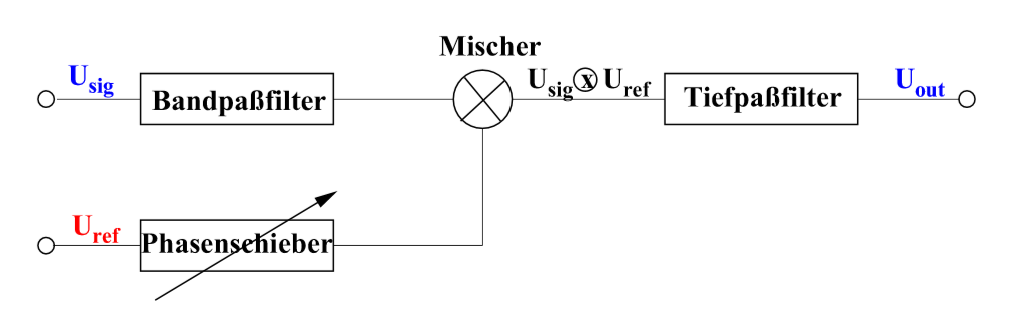
\includegraphics{Bilder/schema.png}
\end{figure}

\noindent Durch das Mischen fällt im Mittel das Rauschen, welches eine ähnliche Frequenz wie die Modulationsfrequenz hat, weg.
Dabei wird die Phase von $U_{ref}$ so angepasst, dass die Phasendifferenz $\increment \varphi=0$ ist.
Angenommen $U_{sig}$ etspricht der Form $U_{sig}=U_0 \sin(\omega t)$ und die Referenzspannung ist eine Rechteckspannung, dann kann Letztere mit der Fourierreihe 
\begin{equation}
    U_{ref}=\frac{4}{\pi} \sum_{k=1}^\infty \frac{1}{k}\sin(k\omega t) \qquad k \in 2n+1 \, n \in \mathbb{N}
    \label{eqn:Fourier}
\end{equation}
beschrieben werden.
Bei dem Produkt der Signale 
\begin{equation}
    U_{sig} \times U_{ref}=\frac{2}{\pi}U_0 \biggl(1-\frac{2}{3}\cos(2\omega t)-\frac{2}{15}\cos(4\omega t)- \frac{2}{35}\cos(6 \omega t)+ \; ...\biggr)
    \label{eqn:Produkt}
\end{equation}
ist erkennbar, dass die Terme nach dem ersten konstanten Term alle höhere Frequenzen besitzen.
Diese fallen für das Ausgangssignal $U_{out}$ wegen dem dafür ausgewählten Tiefpass weg.
Dadurch ist die resultierende Spannung mit
\begin{equation}
    U_{out}=\frac{2}{\pi}U_0
    \label{eqn:konst}
\end{equation}
konstant.
Wenn eine Phasendifferenz zwischen $U_{sig}$ und $U_{ref}$ vorliegt, ist die Ausgangsspannung 
\begin{equation}
    U_{out}=\frac{2}{\pi}U_0 \cos(\varphi).
    \label{eqn:cos}
\end{equation}
